%%%
% Plantilla de Memoria
% Modificación de una plantilla de Latex de Nicolas Diaz para adaptarla 
% al castellano y a las necesidades de escribir informática y matemática%
% Editada por: Mario Román
%
% License:
% CC BY-NC-SA 3.0 (http://creativecommons.org/licenses/by-nc-sa/3.0/)
%%%

%%%%%%%%%%%%%%%%%%%%%%%%%%%%%%%%%%%%%%%%%
% Thin Sectioned Essay
% LaTeX Template
% Version 1.0 (3/8/13)
%
% This template has been downloaded from:
% http://www.LaTeXTemplates.com
%
% Original Author:
% Nicolas Diaz (nsdiaz@uc.cl) with extensive modifications by:
% Vel (vel@latextemplates.com)
%
% License:
% CC BY-NC-SA 3.0 (http://creativecommons.org/licenses/by-nc-sa/3.0/)
%
%%%%%%%%%%%%%%%%%%%%%%%%%%%%%%%%%%%%%%%%%

%----------------------------------------------------------------------------------------
%	PAQUETES Y CONFIGURACIÓN DEL DOCUMENTO
%----------------------------------------------------------------------------------------

%%% Configuración del papel.
% microtype: Tipografía.
% mathpazo: Usa la fuente Palatino.
\documentclass[a4paper, 20pt, dvipsnames]{article}
\usepackage[a4paper,margin=1in]{geometry}
\usepackage[protrusion=true,expansion=true]{microtype}
\usepackage{mathpazo}

% Indentación de párrafos para Palatino
\setlength{\parindent}{0pt}
  \parskip=8pt
\linespread{1.05} % Change line spacing here, Palatino benefits from a slight increase by default


%%% Castellano.
% noquoting: Permite uso de comillas no españolas.
% lcroman: Permite la enumeración con numerales romanos en minúscula.
% fontenc: Usa la fuente completa para que pueda copiarse correctamente del pdf.
\usepackage[spanish,es-noquoting,es-lcroman,es-tabla,,es-nodecimaldot]{babel}
\usepackage[utf8]{inputenc}
\usepackage{fontenc}
\selectlanguage{spanish}


%%% Gráficos
\usepackage{graphicx} % Required for including pictures
\usepackage{wrapfig} % Allows in-line images
\usepackage[usenames,dvipsnames]{color} % Coloring code
%\usepackage{subcaption}
\usepackage{subfig}
\graphicspath{{./fig/}}
\captionsetup{width=0.8\textwidth}

%%% Matemáticas
\usepackage{amsmath}
\usepackage{physics} % para las derivadas parciales
\usepackage[Symbol]{upgreek} %pi

%%% Pseudocódigo
\usepackage[htt]{hyphenat} % Permite salto de líneas en texttt
\usepackage{algorithmicx}
\usepackage[ruled]{algorithm}
\usepackage{algpseudocode}

\newcommand{\alg}{\texttt{algorithmicx}}
\newcommand{\old}{\texttt{algorithmic}}
\newcommand{\euk}{Euclid}
\newcommand\ASTART{\bigskip\noindent\begin{minipage}[b]{0.5\linewidth}}
\newcommand\ACONTINUE{\end{minipage}\begin{minipage}[b]{0.5\linewidth}}
\newcommand\AENDSKIP{\end{minipage}\bigskip}
\newcommand\AEND{\end{minipage}}


%%% Tablas
\usepackage{tabularx}
\usepackage{float}
\usepackage{adjustbox}
\usepackage{booktabs}

% Enlaces y colores
\usepackage{hyperref}
\usepackage[dvipsnames]{xcolor}
\definecolor{webgreen}{rgb}{0,0.5,0}
\hypersetup{
  colorlinks=true,
  citecolor=RoyalBlue,
  urlcolor=RoyalBlue,
  linkcolor=RoyalBlue
}

%%% Código
\usepackage{listings}
\lstset{
  basicstyle=\ttfamily,
  columns=fullflexible,
  %frame=single,
  breaklines=true
}

%%% Gráficas
\usepackage{pgfplots}
\pgfplotsset{compat=1.15}

%%% Bibliografía
\usepackage[backend=biber]{biblatex}
\DefineBibliographyStrings{spanish}{
  urlseen = {Accedido}
}
\addbibresource{citations.bib}


\newcommand{\training}{\textit{training }}
\newcommand{\test}{\textit{test }}
\newcommand{\RF}{\textit{Random Forest }}

\DeclareMathOperator{\acc}{\texttt{accuracy}}

%%% Subsubsection con letras
\renewcommand{\thesubsubsection}{\thesubsection.\alph{subsubsection}}

%%% Itemize, enumitem
\usepackage{paralist}
\usepackage{enumitem}

\usepackage[section]{placeins}
% \makeatletter
% \AtBeginDocument{%
%   \expandafter\renewcommand\expandafter\subsection\expandafter
%     {\expandafter\@fb@secFB\subsection}%
%   \newcommand\@fb@secFB{\FloatBarrier
%     \gdef\@fb@afterHHook{\@fb@topbarrier \gdef\@fb@afterHHook{}}}%
%   \g@addto@macro\@afterheading{\@fb@afterHHook}%
%   \gdef\@fb@afterHHook{}%
% }
% \makeatother


%%% Entornos personalizados
\newenvironment{bloque}[1]
{
\begin{tabular}{|l|}
 \multicolumn{1}{c}{\textbf{\large #1}} \\
 \hline
 \textbf{Capa/bloque} \\
 \hline}
{
 \\\hline
    \end{tabular}   
}

\newenvironment{modelo}[1]
{
\begin{tabular}{ |p{4cm}||p{1.5cm}|p{1.5cm}|  }
 \multicolumn{3}{c}{\textbf{\large #1}} \\
 \hline
 \textbf{Capa/bloque} & \textbf{Entrada} & \textbf{Salida} \\
 \hline}
{
 \\\hline
    \end{tabular}   
}

%----------------------------------------------------------------------------------------
%	TÍTULO
%----------------------------------------------------------------------------------------
% Configuraciones para el título.
% El título no debe editarse aquí.
\renewcommand{\maketitle}{
  \begin{flushright} % Right align
  
  {\LARGE\@title} % Increase the font size of the title
  
  \vspace{50pt} % Some vertical space between the title and author name
  
  {\large\@author} % Author name
  \\\@date % Date
  \vspace{40pt} % Some vertical space between the author block and abstract
  \end{flushright}
}

%% Título
\title{\textbf{Título}\\ % Title
Subtítulo} % Subtitle

\author{\textsc{Autor1,\\Autor2} % Author
\\{\textit{Universidad de Granada}}} % Institution

\date{\today} % Date

%-----------------------------------------------------------------------------------------
%	DOCUMENTO
%-----------------------------------------------------------------------------------------

\begin{document}

%-----------------------------------------------------------------------------------------
%	TITLE PAGE
%-----------------------------------------------------------------------------------------

\begin{titlepage} % Suppresses displaying the page number on the title page and the subsequent page counts as page 1
	
	\raggedleft % Right align the title page
	
	\rule{1pt}{\textheight} % Vertical line
	\hspace{0.05\textwidth} % Whitespace between the vertical line and title page text
	\parbox[b]{0.8\textwidth}{ % Paragraph box for holding the title page text, adjust the width to move the title page left or right on the page
		
		{\Huge\bfseries Proyecto final:\\[0.5\baselineskip] Generación
                  de \LaTeX a partir de imágenes
                  \\[0.5\baselineskip]\\[2\baselineskip]} % Title
		{\large\textit{Curso 2020/21}\\[0.5\baselineskip]Visión por computador\\[1.5\baselineskip] }% Subtitle or further description
		{\Large\textsc{José Antonio Álvarez Ocete, \\Daniel Pozo Escalona}\\[1.5\baselineskip]joseantonioao32@correo.ugr.es\\danipozo@correo.ugr.es,} % Author name, lower case for consistent small caps
		
		\vspace{0.4\textheight} % Whitespace between the title block and the publisher
		
		{\noindent \\[0.5\baselineskip] }\\[\baselineskip] % Publisher and logo
	}

\end{titlepage}

%% Resumen (Descomentar para usarlo)
%\renewcommand{\abstractname}{Resumen} % Uncomment to change the name of the abstract to something else
%\begin{abstract}
% Resumen aquí
%\end{abstract}

%% Palabras clave
%\hspace*{3,6mm}\textit{Keywords:} lorem , ipsum , dolor , sit amet , lectus % Keywords
%\vspace{30pt} % Some vertical space between the abstract and first section

%% Índice
{\parskip=2pt
	\tableofcontents
}
\pagebreak

\newpage

\section{Introducción}

Nuestro objetivo en este trabajo será desarrollar un modelo que, dada una imagen producida al compilar código \LaTeX{} asociado a una fórmula, prediga el código \LaTeX{} que fue utilizado para compilarla. Para ello utilizaremos un esquema codificador - decodificador utilizando transformers.


\section{Bases de datos utilizadas}
\label{sec:datasets}

Las bases de datos para el problema son:

- \textbf{im2latex-100k} (@kanervisto\_anssi\_2016\_56198), y
- \textbf{imlatex-170k} (@im2latex\_170k): contiene 65000 ejemplos, que se añaden a los 100000 de im2latex-100k.

% TODO: revisar que (todas) las referencias están bien puestas.

Ambas bases de datos contienen ambigüedad en los ejemplos, en forma de fórmulas o segmentos de fórmulas que, escritos de distinta forma, producen la misma imagen. Dedicaremos parte del tiempo del proyecto a diseñar formas de normalizar estos datos, para mejorar los resultados. Entraremos en detalle más adelante.

Por ello, las evaluaciones iniciales con modelos de referencia y las finales pueden no ser directamente comparables. Esto lo paliaremos de dos formas: con la base de datos sintética que introducimos a continuación, y evaluando los modelos de referencia en la base de datos normalizada. Además, hay que tener en cuenta que lo relevante en este problema es dar expresiones \LaTeX{} que produzcan las imágenes que se proporcionen al modelo, más que estas coincidan con unas prefijadas.

En la práctica, utilizaremos unicamente im2latex\_170k, ya que contiene a la anterior.

\begin{figure}[H]
	\centering
	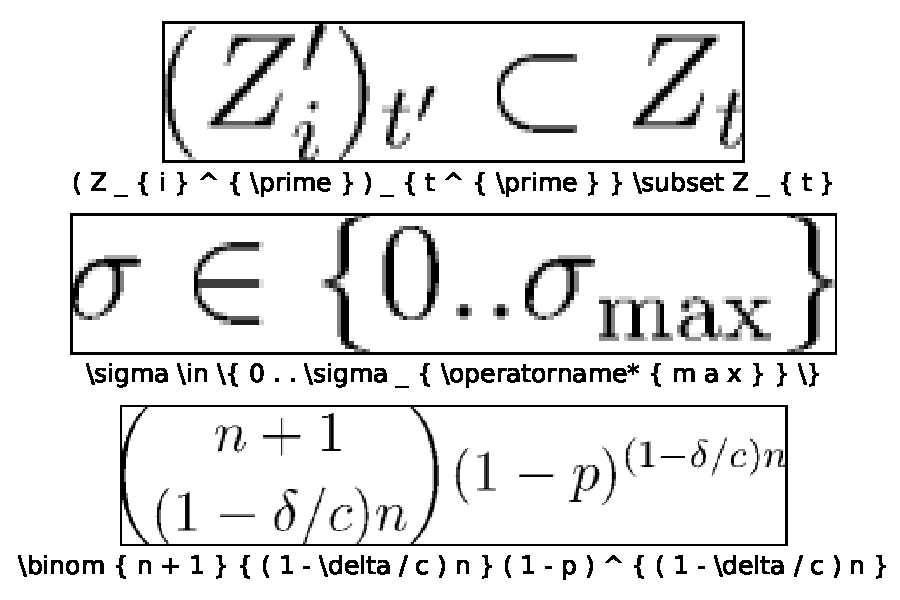
\includegraphics{fig/ejemplo-im2latex.pdf}
	\caption{Tres muestras de im2latex-170k.}
	\label{fig:muestras-1}
\end{figure}


\subsection{Base de datos sintética}

Lo primero que hemos hecho ha sido crear una base de datos similar a las que pretendemos tratar, en la que las fórmulas han sido generadas a partir de una gramática relativamente sencilla, que contiene una cantidad pequeña de símbolos.

Hemos generado 50.000 ejemplos distintos. Los guiones Python que hemos escrito a tal efecto permiten cambiar la gramática y generar conjuntos de datos con cantidades arbitrarias de ejemplos únicos.

Además, esta base de datos puede ser útil para evaluar cambios a la arquitectura o hiperparámetros de forma menos costosa.

\begin{figure}[H]
	\centering
	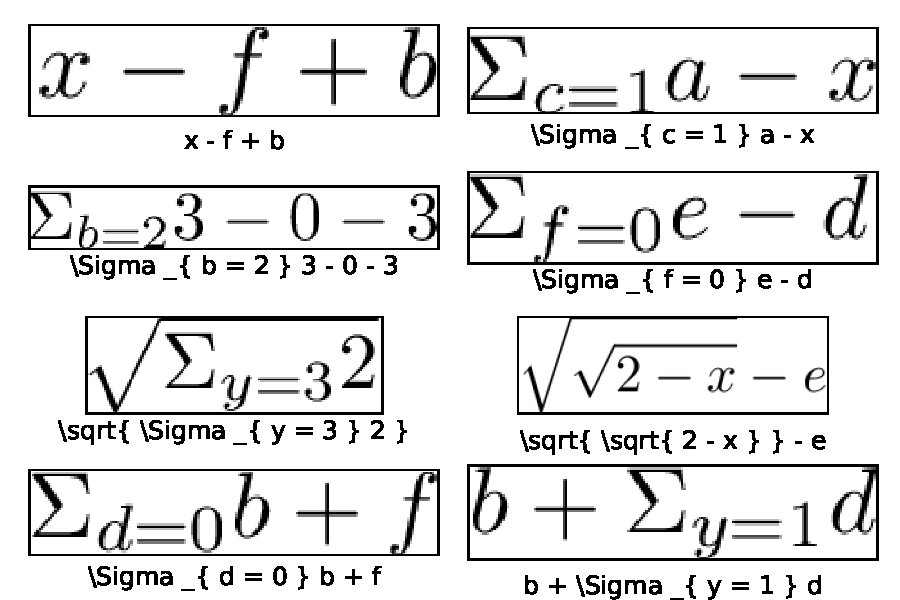
\includegraphics{fig/ejemplo-sintetica.pdf}
	\caption{Muestras de la base de datos sintética.}
	\label{fig:muestras-sintetica}
\end{figure}


\section{Modelo propuesto}

El modelo que proponemos es el siguiente:

- Un codificador, formado por una red convolucional, seguido por un modelo \emph{transformer}.

- Un decodificador \emph{transformer}, que emplea atención multi-cabezal sobre la salida del codificador y sobre una secuencia potencialmente incompleta, para predecir el siguiente token de la fórmula. Es decir, es un modelo de lenguaje condicional que modela $p(x_t | V, x_1, ..., x_{t-1})$, donde $V$ es la salida del codificador.

Utilizaremos una red convolucional para obtener las características de las imágenes de entrada. Este vector de características será la entrada para el modelo codificador-decodificador.

Aunque posteriormente el modelo de referencia que se presenta a continuación sufrirá ciertas variaciones, el esquema general no variará. Este modelo posee un codificador convolucional con tres capas Conv-BN-ELU-MaxPooling y una sola capa de atención en el codificador y en el decodificador.

% TODO: quitar esta proxima linea, que hace que no salga el modelo.
\iffalse
\begin{figure}[h]
	\centering
	
	\subfloat{
		\begin{modelblock}{Codificador convolucional}
			Conv2D-BN-ELU(64 filtros) \\
			MaxPooling2D(2$\times$2) \\
			Conv2D-BN-ELU(64 filtros) \\
			MaxPooling2D(2$\times$2) \\
			Conv2D-BN-ELU(64 filtros) \\
			MaxPooling2D(2$\times$2)
		\end{modelblock}
	}
	\subfloat{
		\begin{modelblock}{Codificador \textit{transformer}}
			Codif. conv. \\
			Codificación de posición \\
			Dropout \\
			Capa de codificador
		\end{modelblock}
	}
	\subfloat{
		\begin{modelblock}{Decodificador \textit{transformer}}
			Embedding \\
			Codificación de posición \\
			Dropout \\
			Capa de decodificador
		\end{modelblock}
	}
	
	\caption{Bloques del modelo de referencia.}
	\label{fig:bloques-referencia}
\end{figure}
\fi
\section{Procesamiento de los datos}

Para las imágenes, el procesamiento que realizamos es redimensionarlas a una altura común, manteniendo la relación de aspecto. Tras esto, eliminamos los ejemplos con imágenes demasiado grandes para ser procesadas por el modelo, debido al coste cuadrático del mecanismo de atención.

Para las fórmulas, utilizamos el [\emph{tokenizer} de TensorFlow](https://www.tensorflow.org/api\_docs/python/tf/keras/preprocessing/text/Tokenizer) para obtener el alfabeto de entrada. Por lo tanto, este no es fijo sino que depende del conjunto de datos. Esto nos permite codificar las fórmulas numéricamente.


\subsection{Lectura eficiente}

Una vez comenzamos a trabajar con la base de datos im2latex descubrimos que ésta no cabía por completo en memoria. De hecho, no cabía ni la un cuarto. De cara a implementar una solución escalable y eficiente a este problema creamos una clase LaTeXrecDataset que hereda de Dataset, de Tensorflow. Esta clase nos permite leer las imágenes conformen el modelo las necesita y, al mismo tiempo, eliminarlas de memoria cuando dejan de hacerlo. Todo esto se procesa de forma automática y muy cómodamente, además de permitirnos implementar \emph{prefetching}. Esto es, lectura anticipada de los datos antes de que hagan falta para acelerar el proceso.

% TODO: no sé si el logging merece la pena comentarlo. Nos llevó su tiempo (tampoco tanto, pero algo) y le añade calidad al código, pero no sé si Nicolás lo verá relevante sinceramente.

Añadimos un sencillo y cómodo sistema de logging a distintos archivos, dependiendo de la información de los mensajes. % TODO completar si decidimos dejarlo.


\section{Características de desarrollo}

% TODO: se requiere urgentemente un nuevo nombre para esta sección porque vaya tela

En esta sección describimos las distintas características implementadas sobre el modelo inicial descrito con anterioridad. Los resultados de las mismas se describen en la sección de experimentos.


\subsection{Eliminación de ambigüedades}

Como ya discutimos en la \hyperref[sec:datasets]{sección de bases de datos}, en este problema encontramos ambigüedad en la salida de los datos. Distintas expresiones $LaTeX$ generar la misma salida o una casi indistiguible en la imagen. Por ejemplo, \emph{\textbackslash sin} y \emph{\textbackslash operatorname\{sin\}}: $\sin(x)$ frente a $\operatorname{sin}(x)$.

Esto hace que el aprendizaje sea  más difícil. El primer cambio que hicimos tras tener un modelo funcional fue eliminar este tipo de ambigüedades en los datos. Cabe aclarar que aunque estemos alterando los datos, la imagen \LaTeX{} obtenida es exactamente la misma en todos estos casos.

Para ello, utilizamos el [\emph{tokenizer} de TensorFlow](https://www.tensorflow.org/api\_docs/python/tf/keras/preprocessing/text/Tokenizer) para generar una lista de tokens de las primeras 60.000 imagénes en la que basarnos. Estudiando esta lista hemos decidido modificar las siguientes ambigüedades, buscando un balance entre implementación sencilla y que merezca la pena porque sean lo suficientemente relevantes:

- Los operadores con nombre más famosos (como seno y máximo), tienen un comando particular en \LaTeX{}: \emph{\textbackslash sin}, y \emph{\textbackslash max}. Utilizaremos estos comandos en vez de los respectivo \emph{\textbackslash operatorname\{sin\}} y \emph{\textbackslash operatorname\{max\}}, siempre que se pueda. Aplicaremos esta misma sustitución para los comandos con un asterisco: \emph{\textbackslash operatorname* \{sin\}}. La lista completa de operadores a  la que le aplicamos essta sustitución es la siguiente: `\emph{\textbackslash sin}, \emph{\textbackslash cos}, \emph{\textbackslash tan}, \emph{\textbackslash arcsin}, \emph{\textbackslash arccos}, \emph{\textbackslash arctan}, \emph{\textbackslash sinh}, \emph{\textbackslash cosh}, \emph{\textbackslash tanh}, \emph{\textbackslash max}, \emph{\textbackslash min}, \emph{\textbackslash exp}, \emph{\textbackslash log}, \emph{\textbackslash ln}, \emph{\textbackslash sup}, \emph{\textbackslash inf}, \emph{\textbackslash lim}, \emph{\textbackslash dim}, \emph{\textbackslash deg}, \emph{\textbackslash ker}, \emph{\textbackslash cot}, \emph{\textbackslash Pr}, \emph{\textbackslash lg}, \emph{\textbackslash arg}, \emph{\textbackslash det}, \emph{\textbackslash vol}.

- El comando \emph{\textbackslash prime} se utiliza en \LaTeX{} para mostar una comilla grande. En caso de utilizarse como exponente (\emph{ \textbackslash \textasciicircum \{ \textbackslash prime \}}) tiene la misma representación gráfica que una comilla simple: \textbf{'}. Sustituiremos la expresión: `\emph{ \textbackslash \textasciicircum \{ \textbackslash prime \}}` por '.

- Los símbolos de llaves `\{` y `\}` se pueden escribir también como `\emph{ \textbackslash brace }` y `\emph{ \textbackslash rbrace }` respectivamente. Los sustituiremos por la versión más corta que es, además, más general ya que se puede utilizar tanto en modo texto como en modo matemáticas.

- El símbolo de la daga se puede escribir en $LaTex$ utilizando tanto `\emph{ \textbackslash dagger }` como `\emph{ \textbackslash dag }`. Aunque este símbolo apenas aparece en nuestras fórmulas, añadir esta sustitución es una línea extra que no añade complejidad ninguna. Utilizaremos su versión más corta.

- Finalmente, la tipografía aplicada al utilizar `\emph{\textbackslash cal}` y `\emph{\textbackslash mathcal}` es exactamente la misma aunque su sintaxis es distinta. `\emph{\textbackslash cal}` se utiliza para palabras o letras sueltas: `\emph{\textbackslash prime} A`; mientras que `\emph{\textbackslash mathcal}` se utiliza para expresiones más complejas: `\emph{\textbackslash mathcal} \{ sin \textasciicircum \{ 2 \} ( x ) \}`. Puesto que el uso de `\emph{\textbackslash cal}` está deprecado y `\emph{\textbackslash mathcal}` es más general, utilizaremos este último, reajustando la sintaxis conforme sea necesario.


\subsection{Atención eficiente}

Uno de los principales escollos que hemos encontrado ya desde el trabajo preliminar en este proyecto es el enorme consumo de memoria del modelo \emph{transformer}. Esto se debe a que, en cada capa de atención, se ha de calcular la matriz de atención, de tamaño cuadrático en la longitud de la secuencia procesada. En el caso de las características provenientes de la imagen, esta secuencia puede alcanzar longitud 500.

Recientemente, se han propuesto múltiples alternativas para aproximar el mecanismo de atención de forma más eficiente (@tay2020efficient). En la tabla 1 de este artículo de revisión se encuentran listadas todas las alternativas, junto con algunas características de las mismas.

Hemos seleccionado, de entre las que permiten emplear un decodificador, la atención rápida mediante el mecanismo FAVOR+ (@choromanski\_rethinking\_2020), la hemos implementado y probado.


\subsection{Codificación posicional 2-dimensional}

La capa de \emph{self attention} en la que se basan los bloques transformers sigue un modelo de conexión `todos con todos`, por lo que pierde la información posicional de los elementos que recibe. Es por ello que se añade codificación posicional, para añadir artificalmente dicha información de la posición de cada palabra.

% TODO: No estoy nada seguro de querer poner esta foto y essta explicación creo que anda un poco cogida con pinzas, una revisión técnica no le viene mal.

\begin{figure}[H]
	\centering
	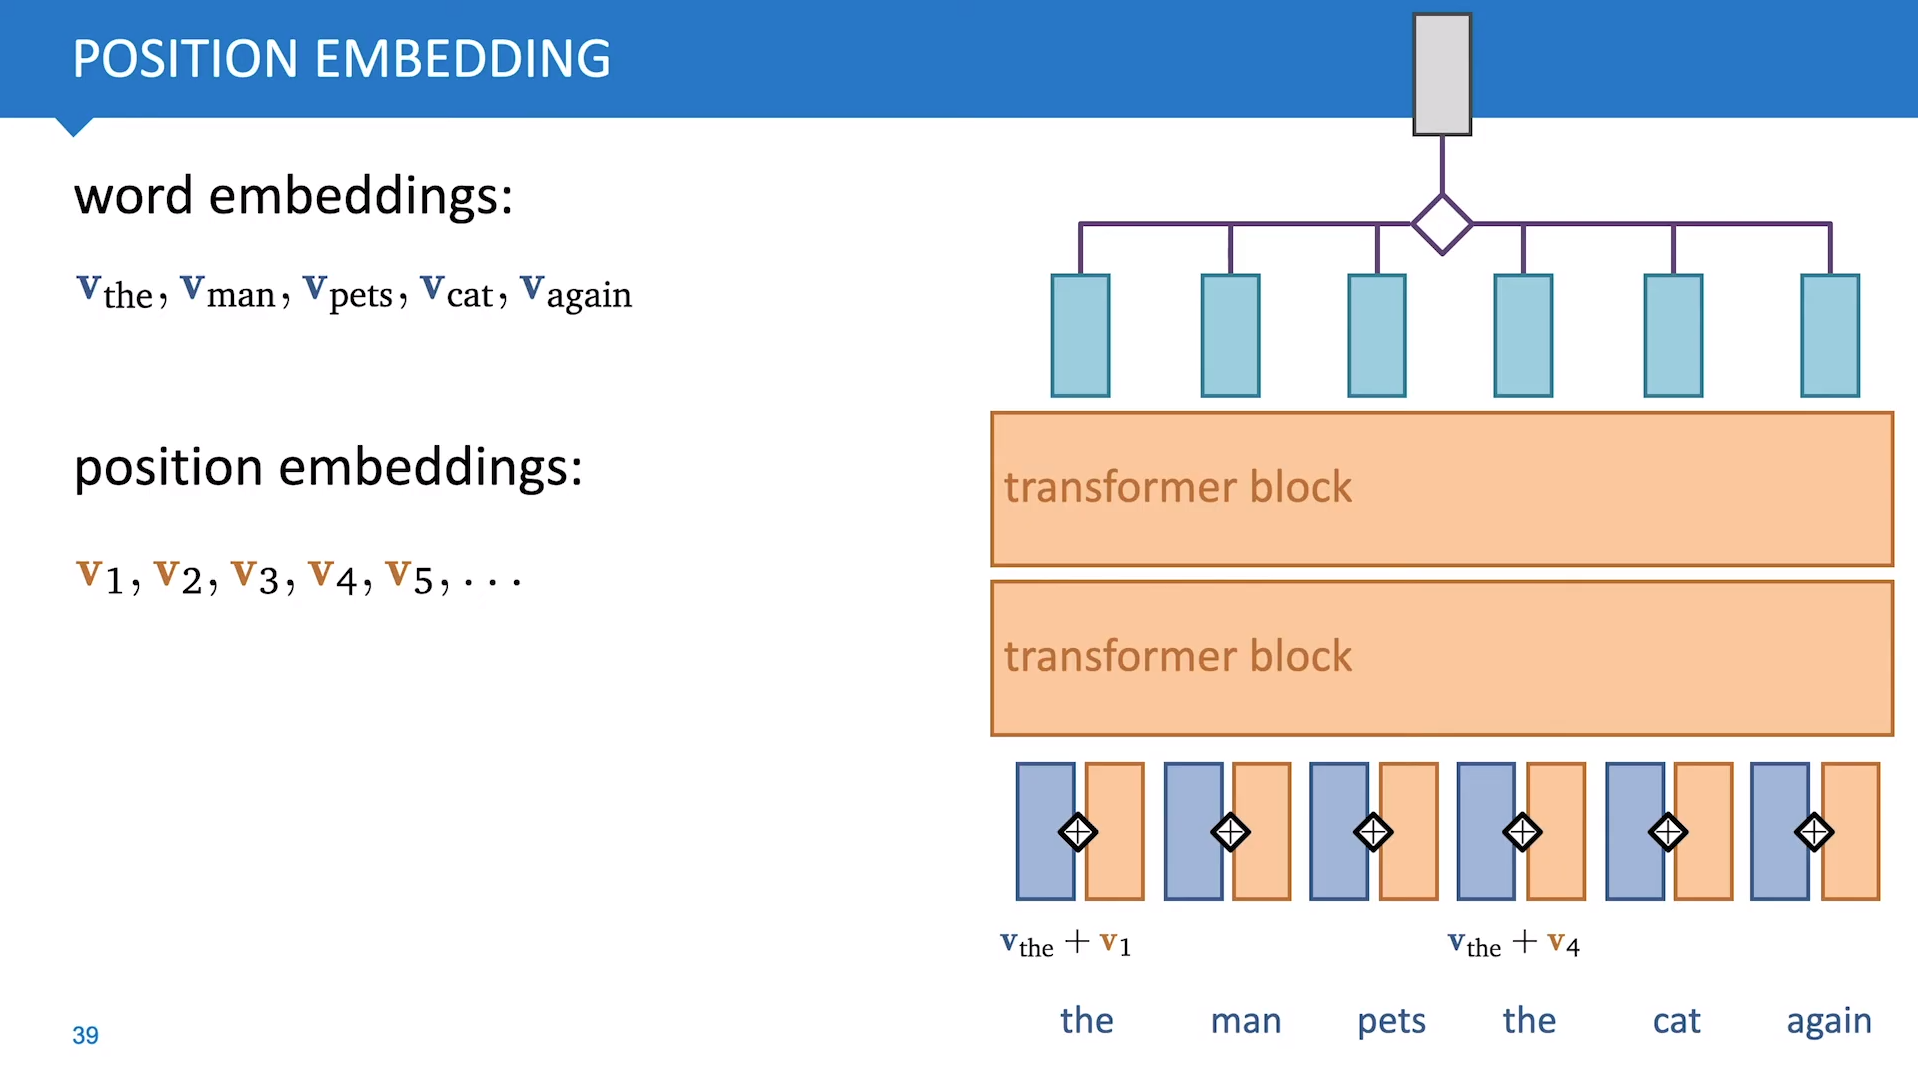
\includegraphics[scale=0.15]{fig/positional}
	\caption{Diseño de codificación posicional.}
\end{figure}

% TODO: Añadir a las refs:
% https://www.youtube.com/watch?v=oUhGZMCTHtI\&list=PLIXJ-Sacf8u60G1TwcznBmK6rEL3gmZmV&index=2

En nuestro caso particular, añadimos esa codificación posicional también a la salida de nuestra red convolucional con las características de la imagen obtenidas. A pesar de que dicha imagen tenga dos dimensiones, se aplana en una única dimensión antes de añadirle esta información, perdiendo la posición relativa en la imagen en el proceso.

Para paliar esta pérdida de información hemos implementado codificación posicional 2-dimensional, utilizando así la información relativa de las características al completo.

% TODO: aqui vendria super bien añadir la ref de donde hemos sacado la implementacion de codificación posicional:
% https://github.com/wzlxjtu/PositionalEncoding2D/blob/master/positionalembedding2d.py

\subsection{Métrica BLEU}

Hacia el final del desarrollo hemos implementado la [métrica BLEU](https://en.wikipedia.org/wiki/BLEU) para evaluar de forma más intuitiva los resultados obtenidos. Esta métrica nos da una estimación de cuanto se parecen dos cadenas de tokens. Suele utilizarse para comparar cuán buena es una traducción de lenguaje a otro, y la utilizaremos en el último experimento.

% Referencia: [tensor2tensor](https://github.com/tensorflow/tensor2tensor/blob/master/tensor2tensor/utils/bleu\_hook.py#L132).


\section{Experimentos}

\subsection{Experimentos sobre Toy}

\subsubsection{Vanilla}
\subsubsection{ResNet}
\subsubsection{Atención Rápida}

\subsection{Experimentos sobre Im2Latex}

\subsubsection{Vanilla}

\subsubsection{Eliminar ambigüedades}

\subsubsection{Atención rápida}

\subsubsection{ResNet}

\subsubsection{Codificación positional 2-dimensional}

\subsubsection{Learning rate modificado}

\subsection{Experimentos finales}

\subsubsection{Big boy}

\subsubsection{Bigger boy}

\subsubsection{Lattest boy (estudio sobre test)}








%%%%%%%%%%%%%%%%%%%%%%%%%%%%
\printbibliography
\end{document}
